% !TEX root = BA-Bauer

\newpage
\section{Hardware}
In den folgenden Kapiteln wird auf die in dieser Arbeit verwendete Hardware eingegangen. Zunächst wird das grundlegende Pinzip der Schaltung erläutert. Daraufhin werden die Bestandteile bzw. Module im Einzelnen näher erläutert und deren Funktionsweise und Funktion in der Gesamtschaltung erklärt. Abschließend wird erläutert, wie die abstrakte Schaltung in ein Platinendesign überführt und wie diese in einem Gehäuse plaziert wird. Die Datenblätter der Hardwarekomponenten befinden sich im Anhang \ref{CD-Anhang}.
% !TEX root = BA-Bauer

\subsection{Schaltungsprinzip}

In diesem Kapitel wird auf das grundlegende Prinzip der gesamten Schaltung eingegangen. Auf die einzelnen Komponenten und deren benötigte Beschaltung wird in den folgenden Kapiteln eingegangen. Generell wird bei der Entwicklung der Schaltung darauf geachtet, dass möglichst keine fertigen Modulbausteine verwendet werden. Dadurch ergibt sich in der Regel ein Preisvorteil und vereinfacht die industrielle Bestückung der Platine, in Hinsicht auf eine Serienproduktion. %(Quelle?)
Abbildung \ref{fig:Schaltungsrinzip} zeigt das grundlegende Prinzip der Schaltung. Auf der linken Seite befindet der Benutzer des Gerätes. Er bedient das Gerät durch seine Eingaben und erhält entsprechende Rückmeldungen zurück. Die grüne Fläche spiegelt das Gerät wieder, welches mit der DMX-Quelle bzw. der DMX-fähigen Lichttechnik auf der rechten Seite kommuniziert. Im Folgenden wird auf die Bestandteile des Gerätes eingegangen.
\begin{figure}[h]
	\includegraphics[width = \textwidth]{Schaltungsprinzip}
	\caption{Schaltungsprinzip}
	\label{fig:Schaltungsrinzip}
\end{figure}\\
\textbf{Mikrocontroller (MCU)}\\
Der Mikrocontroller, im Folgenden MCU genannt, bildet den Mittelpunkt der Schaltung. Die auf ihm ausgeführte Software steuert die Benutzerschnittstelle (UI), speichert und ruft Daten vom Speicher ab und sendet und empfängt die DMX-Daten. Aufgrund der hohen Anforderungen an den MCU wird bei der Entwicklung ein besonderes Augenmerk auf ihn und seine Beschaltung gelegt. Die Auswahl des MCUs orientiert sich an dem in der Praxisprojektarbeit verwendeten Mikrocontroller, da dessen Funktionsfähigkeit bereits erwiesen ist.\\
\newline
\textbf{Spannungsversorgung (Power)}\\
Alle Komponenten werden von einer USB-Schnittstelle mit Spannung versorgt. Da das Gerät eigenständig verwendet werden soll, werden über die Schnittstelle keine Daten übertragen. Die Schnittstelle liefert 5\,V Spannung \cite[S. 44]{USB-Battery}, welche in die benötigten Spannungen transformiert werden. Besonders kritisch ist die Spannungsversorgung des MCUs, denn unter normalen Betriebsbedingungen darf die Versorgungsspannung nur soweit einbrechen, dass der MCU weiterhin den darauf befindlichen Programmcode fehlerfrei ausführen kann.\\
\textbf{Benutzerschnittstelle (UI)}\\
Damit der Benutzer das Gerät bedienen kann, ist ein Informationsfluss in zwei Richtungen erforderlich. Zum einen müssen Eingaben durch den Benutzer erfasst werden, zum anderen muss das Gerät dem Benutzer eine Rückmeldung über Fehler oder den aktuellen Status geben können. Für die Benutzereingaben werden mehrere Taster und ein Drehgeber (Encoder) verwendet. Durch den Einsatz von Tastern können präzise und zeitgenaue Eingaben vom Benuter vorgenommen werden, an Stellen an denen es nötig ist, zum Beispiel beim Starten einer Wiedergabe. Der Encoder hingegen bietet die Möglichkeit viele Eingaben in kurzer Zeit zu tätigen, zum Beispiel wenn die Aufnahmezeit eingestellt wird.\\
\newline
\textbf{RS485}\\
Die RS485-Schnittstelle ist die Verbindung zwischen DMX-Quelle/Senke und dem MCU. Diese ist notwendig ist, da der MCU keine RS485 konformen Signalpegel liefern, oder auswerten kann. Zudem werden durch die Schnittstelle die DMX-Leitungen galvanisch von der restlichen Schaltung getrennt. Spannungs- und Stromspitzen ausgehend von den DMX-Leitungen können so die Schaltung nicht beeinträchtigen oder beschädigen.\\
\newline
\textbf{Speicher (SD-Karte)}\\
Damit ein sinnvoller Einsatz des Gerätes möglich ist, müssen die aufgenommenen Daten auch nach einem Neustart des Geräts verfügbar sein. Deswegen ist die Sicherung auf einem Speichermedium notwendig. In der vorangegangen Praxisprojektarbeit wurde bereits gezeigt, dass der Einsatz einer SD-Karte für diesen Zweck geeignet ist. Die Verwendung einer SD-Karte ermöglicht dem Benutzer außerdem eine gewisse Sicherheit in Bezug auf den Schutz der Daten. Eine Sicherungskopie der Daten kann einfach auf einem PC erstellt werden. Zudem können für verschiedene Einsatzgebiete verschiedene SD-Karten verwendet werden.
% !TEX root = BA-Bauer

\subsection{STMicroelectronics STM32F446ZE}
\label{sec:STM}
Aufgrund der aktuellen Corona-Pandemie und einer damit einhergehenden Siliziumchip-Knappheit kann für die Entwicklung nicht der gleiche MCU verwendet werden, wie in der Praxisarbeit. Die Eckdaten beider Mikrocontroller sind allerdings ähnlich. Abbildung \ref{fig:MCU_pinout} zeigt die Pinbelegung des Chips. Insgesamt stehen bis zu 20 Schnittstellen und 114 interruptfähige Ein- und Ausgangsports, von denen 112 5\,V-tolerant sind, zur Verfügung. Der interne 512\,kBytes große Flash-Speicher und 128\,kByte SRAM bieten genügend Kapazität für einen großen Programmcode, sowie genügend Platz für Heap und Stack. Der STM32F446ZE arbeitet mit einer maximalen Taktfrequenz von 180MHz und basiert auf einem \textit{Arm\textsuperscript{®} 32-bit Cortex\textsuperscript{®}-M4} Prozessor \cite[S. 1]{STM32F446ZE_Datasheet}.
\begin{figure}[!htb]
	\begin{center}
		\includegraphics[scale = 0.4]{STM32F446ZE_pinout}
		\caption{STMicroelectronics STM32F446ZE Mikrocontroller Pinout \cite[S. 41]{STM32F446ZE_Datasheet}}
		\label{fig:MCU_pinout}
	\end{center}
\end{figure}\\
\newline
\hspace{-5mm}\textbf{Spannungsversorgung}\\
Die Spannungsversorgung des MCUs ist besonders kritisch, da eine einbrechende Spannung zu Fehlern bei der Ausführung des Programmcodes oder sogar zu einem kurzzeitigen Ausfall und Neustart des MCUs führen kann. Bei steigenden Schaltfrequenzen des MCUs wirken die Leiterbahnen auf der Platine induktiv, wodurch möglicherweise nicht schnell genug genügend Strom geliefert werden kann, was zu einem Einbruch der Spannung führen kann. Um dem entgegenzuwirken werden sogenannte Stützkondensatoren möglichst nah an den Versorgungsspannungs-Pins ($V\textsubscript{DD}$ und $V\textsubscript{SS}$) des MCUs platziert. Benötigt der MCU kurzzeitig einen großen Strom, so entlädt sich der Kondensator. Durch die kurze Distanz zum MCU muss der Strom über eine kürzere Strecke der Leiterbahn fließen, was eine niedrige Induktivität zur Folge hat. Aus dem Datenblatt \cite{F446RM} des MCUs kann die Dimensionierung der Stützkondensatoren entnommen werden. Insgesamt werden elf Pin-Paare, bestehend aus $V\textsubscript{DD}$ (3,3\,V) und $V\textsubscript{SS}$ (0\,V), mit 0,1\,$\mu$F Kondensatoren parallel verbunden.\\
\newline
\textbf{Taktgeber (Clock)}\\
Der MCU verfügt über einen internen Hochgeschwindigkeits-Oszillator \textit{High-Speed-Internal-Clock} (HSI) und einen Niedergeschwindigkeits-Oszillator \textit{Low-Speed-Internal-Clock} (LSI). Die HSI schwing mit einer Frequenz von 16\,MHz und ist werksseitig auf eine Abweichung der Schwingfrequenz von einem Prozent kalibriert. Um die maximale Taktfrequenz des Prozessors zu erreichen, wird eine interne Phasenregelschleife \textit{phase-locked loop}(PLL) eingesetzt. Durch die PLL kann ein Vielfaches der Oszillatorfrequenz erzeugt werden, wobei die Stabilität der Schwingung nicht eingeschränkt wird \cite[S. 270]{Ehrhardt1992}. Eine weitere Möglichkeit die Taktfrequenz zu generieren, ist die Verwendung eines externen Oszillators \textit{High-Speed-External-Clock} (HSE). Der in dieser Arbeit verwendete externe Quartz schwingt mit einer Frequenz von 25\,MHz und hat dabei eine Genauigkeit von 30\,ppm. Das entspricht einer maximalen Abweichung von ca. \(30*10^{-6}\)\,\%, also einer deutlich geringeren Abweichung im Vergleich zum internen Oszillator. Da für die Aufnahme und Wiedergabe der DMX-Daten möglichst genaue Zeitabstände benötigt werden, wird der externe Quartz verwendet.
\begin{figure}[!h]
	\begin{center}
			\includegraphics[scale=1]{Schaltung-Quartz}
			\caption{Beschaltung Quartz}
			\label{fig:Quartz}
	\end{center}
\end{figure}\\
Abbildung \ref{fig:Quartz} zeigt die Beschaltung des externen Quartzes. Er wird parallel zu dem Eingang $OSC\_IN$ und dem Ausgang $OSC\_OUT$ des MCUs geschaltet. Zwischen dem Ein- und Ausgang des MCUs befindet sich ein integriertes \textit{Nicht-Gatter} (Inverter) \cite[S. 11]{OscillatorAN}, welches bei einem Schaltvorgang hohe Ströme ausgeben kann. Damit kein Schaden an Quartz und MCU entsteht, wird der maximal fließende Strom durch den Widerstand \textit{R1C} am $OSC\_OUT$-Pin begrenzt. Aus Symmetriegründen befindet sich ein 0\,$\Omega$-Widerstand am $OSC\_IN$-Pin, der dafür sorgt, dass auf beiden Seiten des Quartzes die gleichen Übergangskapazitäten der Lötstellen vorhanden sind. Der Quartz wird mithilfe von zwei Lastkapazitäten mit dem 0\,V Potential verbunden. Der Wert der Kapazitäten \textit{$C_{L1}$} und \textit{$C_{L2}$} lässt sich mit folgender Formel berechnen.
\begin{equation}
		C_L = \frac{C_{L1} * C_{L2}} {C_{L1} + C_{L2}} + C_s \cite[S. 12]{OscillatorAN}
\end{equation}
\textit{$C_L$} wird vom Hersteller des Quartzes vorgegeben und beträgt in diesem Fall 18\,pF \cite{QuartzMN}. \textit{$C_S$} ist die Kapazität der Lötstellen und Leiterbahnen zwischen dem Quartz und dem MCU, welche mit 5\,pF angenommen wird. Um möglichst wenig verschiedene Bauteile verwenden zu müssen, erhalten in der Regel die Kapazitäten $C_{L1}$ und $C_{L2}$ die gleiche Wertigkeit, wodurch die Formel wie folgt vereinfacht werden kann.
\begin{equation}
	C_{L1} =  C_{L2} = 2(C_L - C_S)
\end{equation}
Laut der Formel müssen $C_{L1}$ und $C_{L2}$ eine Kapazität von 26\,pF aufweisen. Da Kondensatoren mit dieser Kapazität nur schwer erhältlich sind wird eine marktüblichere Kapazität von 27\,pF verwendet.\\
\newline
\textbf{Serial Wire Debug-Schnittstelle}\\
Im Auslieferungszustand des MCUs befindet sich keine Software auf diesem. Mit einem Entwicklungsboard, wie es in der Praxisarbeit verwendet wurde, kann eine Software einfach über eine USB-Schnittstelle auf den MCU übertragen werden, da auf dem Entwicklungsboard ein sogenannter $programmer$ verbaut ist. Das in der Praxisarbeit verwendete Entwicklungsboard bietet die Möglichkeit, einen Teil der Platine abzutrennen und als eigenständigen $programmer$ zu verwenden, mit dem die Software mithilfe der \textit{Serial Wire Debug}-Schnittstelle (SWD-Schnittstelle) auf den MCU übertragen werden kann \cite[S.18-19]{F446RE_UM}. Die SWD-Schnittstelle ermöglicht das Übertragen der Software und das Debuggen\footnote{Analyse und Fehlerbehebung von Programmcode} des Codes während der Laufzeit. Für die Datenübertragung zwischen MCU und PC werden nur zwei Verbindungen benötigt. Über die \textit{serial wire data}-Leitung werden die Daten gesendet, wohingegen die \textit{serial wire clock}-Leitung den Takt des Datenstroms angibt. Soll ein neuer Programmcode auf den MCU übertragen werden, so muss er zunächst in einen speziellen Modus versetzt werden, um den Programmspeicher beschreiben zu können. Dazu muss der MCU neugestartet werden und beim Start des MCUs am $BOOT0$-Pin ein High-Pegel anliegen. Sobald die Übertragung beendet ist, muss der MCU ein weiteres Mal neugestartet werden, um den Programmcode auszuführen, jedoch muss beim Start nun ein Low-Pegel am $BOOT0$-Pin anliegen. Das Anlegen der entsprechenden Pegel am $BOOT0$-Pin sowie der Neustart können per Hand durchgeführt werden, allerdings kann diese Aufgabe auch vom $programmer$ übernommen werden. Dafür müssen zwei weitere Verbindungen für den $BOOT0$-Pin und $NRST$-Pin vorhanden sein. Zuletzt ist außerdem eine Verbindung der 0\,V-Potentiale notwendig, da es sich bei allen Signalen um spannungsbezogene Signale handelt. Optional kann der MCU mit einer weiteren Verbindung vom $programmer$ mit 3,3\,V Spannung versorgt werden.\\
\newline
\textbf{NRST- und BOOT0-Pin}\\
Unter den 144 Pins des MCUs befinden sich unter anderem, wie bereits im vorigen Abschnitt erwähnt, der $NRST$- und $BOOT0$-Pin. Beide Pins sind mit externen Tastern beschaltet, um Fehler bei den Verbindungen zwischen MCU und $programmer$ zu kompensieren. Außerdem kann das Programm mit dem Betätigen eines Tasters neugestartet werden, was bei der Programmierung von Vorteil ist. Für den verkaufsfertigen Zustand des Gerätes werden die Taster allerdings nicht benötigt und können weggelassen werden. 
% !TEX root = BA-Bauer
\newpage
\subsection{Maxim Integrated MAX14945EWE+ RS485 Treiberchip}

Für das Senden und Empfangen von DMX-Daten wird eine galvanisch getrennte RS485-Schnittstelle benötigt \cite[S.6-8]{Bauer2021}. Der Einsatz von einzelnen Optokopplern und einem RS-485-Treiberchip, wie in der vorangegangenen Praxisarbeit, benötigt viel Platz auf der Platine. Außerdem bietet er ein hohes Fehlerpotential, da ingesamt vier ICs\footnote{enlg. $integrated\ circuit$: Integrierter Schaltkreis} auf die Platine aufgebracht werden müssen. Potentielle Fehlerquellen sind eine hohe Anzahl an Lötstellen der ICs und deren Beschaltung, sowie die Leiterbahnen zwischen den einzelnen Komponenten. Jedes Stück Leiterbahn kann Störungen in den Rest der Schaltung streuen, was zu Fehlern in kritischen Teilen der Schaltung führen kann, beispielsweise der SD-Karte. Die Lösung dieses Problems ist der intern galvanisch getrennte Treiberchip \textit{MAX14945EWE+} der Firma \textit{Maxim Integrated}.
\begin{figure}[h]
	\begin{center}
		\includegraphics[width=.7\linewidth]{MAX_typical_mark}
		\caption{MAX14945EWE+ Typical Application Circuit \cite[s.19]{MAX14945MN}}
		\label{fig:MAXfd}
	\end{center}
\end{figure}
Abbildung \ref{fig:MAXfd} zeigt den schematischen Aufbau des Treiberchips inklusive dessen typischer Beschaltung. Im blau markierten Bereich befindet sich die galvanische Trennung des Chips. Die gestrichelte Linie in der Mitte markiert die Trennung der Seiten $A$ und $B$. Die Funktionen der Pins können Tabelle \ref{tab:MAX_pins} entnommen werden. Die linke Seite ($A$ Seite) ist dem Mikrocontroller zugewandt und wird mit dem 5\,V Potential der USB-Schnittstelle versorgt und mit einem 0,1\,$\mu$F und 1\,$\mu$F Kondensator in Parallelschaltung gestützt. Die Kondensatoren sollen laut Datenblatt möglichst nah am Treiberchip platziert werden. Pin $TXD$ wird mit dem Ausgang, Pin $RXD$ mit dem Eingang der UART-Schnittstelle des MCUs verbunden. Zum aktivieren des Senders oder Empfängers des Treibers muss ein entsprechender Logikpegel an den Pins $DE$ und $\overline{RE}$ anliegen. Da die Logik des Pins zum Aktivieren und Deaktivieren des Empfängers invertiert ist, können beide Pins kurzgeschlossen werden und mit einem Ausgang des MCUs verbunden werden. Ein interner pulldown-Widerstand an beiden Pins ermöglicht die direkte Verbindung zum MCU ohne weitere Beschaltung. Die rechte Seite ($B$ Seite) des Treiberchips muss, um die galvanische Trennung zu gewährleisten, mit einer entsprechend getrennten Spannungsquelle versorgt werden. Diese wird mithilfe eines DC/DC Konverters, der die von der USB-Schnittstelle eingehenden 5\,V isoliert und am Ausgang wieder ausgibt \cite{DC_MN}, erzeugt. Um eine möglichst stabile Spannungsversorgung zu gewährleisten, wird der im Treiberchip interne $low-dropout$-Spannungsregler vewendet, wodurch Pin $V_{DDB}$ als Ausgang der stabilisierten Spannung fungiert. Pin $V_{DDB}$ und $V_{LDO}$ werden mit jeweils einem 0,1\,$\mu$F und 1\,$\mu$F Kondensator parallel mit $GNDB$ verbunden.
\begin{table}[h]
	\begin{center}
			\caption{Pinbeschreibung MAX14945EWE+ \cite[S.12-13]{MAX14945MN}}
		\begin{tabular}{l | l}
			\textbf{Pin} & \textbf{Funktion}\\
			\hline
			$TXD$ & serieller Dateneingang\\
			$RXD$ & serieller Datenausgang\\
			$DE$ & 1: Sender aktivieren, 0: Sender deaktivieren\\
			$\overline{RE}$ & 1: Empfänger deaktivieren, 0: Empfänger aktivieren\\
			$\overline{SBA}$ & 1: $B$ Seite inaktiv, 0: $B$ Seite funktionsfähig\\
			$A$ \& $B$ & symmetrischer Treiberausgang\\
			$V_{DDA}$ \& $GNDA$ & Spannungsversorgung $A$ Seite\\
			$V_{DDB}$ \& $GNDB$ & Spannungsversorgung $B$ Seite\\
			$V_{LDO}$ & Spannungsregler Eingang $B$ Seite
		\end{tabular}
	\label{tab:MAX_pins}
	\end{center}
\end{table}
%Abbildung \ref{fig:MAXfd} zeigt den schematischen Aufbau des Treiberchips. Die gestrichelte Linie zeigt die galvanische Trennung im inneren des ICs. Auf der linken Seite ($A$ Seite) befindet sich der serielle Eingang ($TXD$) und Ausgang ($RXD$) sowie die Pins $DE$ zum aktivieren und $\overline{$$RE$} deaktivieren des Treibers. Der invertierte Ausgang $\overline{SBA}$ gibt einen low-Pegel aus wenn die rechte Seite (B-Seite) des ICs mit Spannung versorgt ist und funktioniert. Der eigentliche Treiber, sowie dessen symmetrischer Ein- und Ausgang ($A$ und $B$) befinden sich auf Seite $B$. Außerdem finden sich insgesamt 5\,Pins für die Spannungsversorgung des ICs. Um eine vollständige galvanisch entkopplung zu garantieren muss die Spannungsversorgung der $A$ und $B$ Seite auch galvanisch entkoppelt sein. Aus diesem Grund gibt es zwei Pin-Paare, bestehend aus $VDD$ \& $GND$, für Seite $A$ und $B$. Zusätzlich steht auf Seite $B$ ein interner \textit{low-dropout} Spannungsregler (LDO\footnote{Hochempfindliche Schaltung zur linearen Regelung einer spezifischen Spannung. \cite{LDO}}) zur Versorgung der Seite $B$ zur Verfügung. Die galvanisch entkoppelte Spannungsversorgung wird mithilfe eines DC/DC-Konverters mit 5\,V Ein- und Ausgang erreicht. Gespeist wird der Konverter direkt von der USB-Buchse. Seite $B$ benötigt eine Versorgungsspannung zwischen 4,68\,V und 14\,V zwischen Pin $VLDO$ und $GNDB$, Seite $A$ eine Spannung zwischen 1,71\,V und 5,5\,V zwischen Pin $VDDA$ und $GNDA$ \cite[s. 2]{MAX14945MN}. Um Stromspitzen und den damit einhergehenden mögichen Spannungseinbruch aufzufangen werden jeweils zwei Stützkondensatoren mit einer Kapaität von 100\,nF und 1\,$\mu$F zwischen den Versorgungspins geschaltet. 
%-Preistechnis kein Nachteil gegenüber einzelnem Treiber und Optokopplern\\
%-Galvanisch getrennte Spannungsversorgung nach wie vor notwendig\\
% !TEX root = BA-Bauer

\subsection{Encoder}
\label{sec:Encoder}
Für die Benutzereingaben sind Taster und vor allem ein Encoder wichtig. Taster ermöglichen eine zeitlich präzise Eingabe, wohingegen ein Encoder viele Eingaben in kurzer Zeit ermöglicht. Möchte ein Benutzer eine Aufnahmezeit von 55 Sekunden einstellen, so müsste er 55 Mal einen Taster betätigen, mit einem Encoder reichen wenige Umdrehungen dafür aus. In diesem Kapitel wird auf das Funktionsprinzip und die Beschaltung des verwendeten Encoders eingegangen.\\
%Formulierung: Raster bei den Umdrehung ->24
Ein Encoder besteht im einfachsten Sinne aus zwei Schaltern, wie Abbildung \ref{fig:Encoder-Schaltung} zeigt. 
\begin{figure}[h]
	\begin{center}
		\includegraphics[scale = 1.2]{Encoder-Schaltung-Eagle}
		\caption{Encoder Schaltung \cite{EncoderMN}}
		\label{fig:Encoder-Schaltung}
	\end{center}
\end{figure}
Die Schalter sind auf der einen Seite intern miteinander verbunden (\textit{Terminal C}) und werden auf das 0\,V Potential geschaltet. Die andere Seite der Schalter wird direkt über \textit{Terminal A} und \textit{Terminal B} nach außen geführt. 
%Jeweils ein exerner 10\,k$\Omega$ Pull-Up-Widerstand (R1 und R3) zieht die Ausgänge auf die Betriebsspannug von 5\,V. Ist der Schalter geöffnet, so fließt kein Strom und folglich fällt keine Spannung am Pull-Up-Widerstand ab. Am entsprechenden Terminal können 5\,V gegenüber der Masse gemessen werden. Ist der Schalter geschlossen so fällt die gesamte Spannung am Widerstand ab und am entsprechenden Terminal liegt nun Masse-Potential an. 
Beide Terminals werden mit jeweils einem 10\,k$\Omega$ Pull-Up-Widerstand ($R1$ und $R2$) auf die Betriebsspannung von 5\,V gezogen. Gleichzeitig wird der Strom, der fließt wenn ein Schalter geschlossen ist, begrenzt. Der Hersteller des Encoders empfiehlt das Beschalten des Encoders mit zwei CR-Tiefpassfiltern, um hochfrequente Schaltvorgänge zu filtern. Bei einem Schaltvorgang können die Kontakte des Schalters mechanisch schwingen (Prellen) und dadurch mehrfach hintereinander öffnen und schließen \cite[S. 67]{TechInfo}, wodurch mehrfache Eingaben getätigt werden, obwohl der Encoder nur um einen Schritt gedreht wurde. Die Signale des Encoders werden an Punkt A und B in Abbildung \ref{fig:Encoder-Schaltung} entnommen und über zwei Leiterbahnen zum MCU geführt. Ist ein Schalter geöffnet, so wird die Kapazität des CR-Filters geladen und die an ihm abfallende Spannung erhöht sich bis zur Betriebsspannung von 5\,V. Wird der Schalter nun geschlossen, so entlädt sich der Kondensator in Richtung des entsprechenden Terminals. Die Spannung an der Kapazität sinkt bis zum 0\,V-Potential. Fängt ein Schalter an zu schwingen, reicht die Zeit zum Laden bzw. Entladen der Kapazität nicht aus, um eine Pegeländerung zu erzielen. 
\begin{figure}[h]
	\includegraphics[width=\linewidth]{Encoder-signal}
	\caption{Encoder-Signal bei Drehung im Uhrzeigersinn}
	\label{fig:Encoder-signal}
\end{figure}
Wenn der Encoder gedreht wird, schließen und öffnen die internen Schalter versetzt zueinander. Abbildung \ref{fig:Encoder-signal} zeigt die ausgehenden Signale \textit{A} und \textit{B} im zeitlichen Verlauf bei einer gleichmäßigen Rotationsgeschwindigkeit. Durch den versetzten Rhythmus der beiden Schalter kann die Drehrichtung bestimmt werden, indem eines der beiden Signale betrachtet wird, in diesem Beispiel Signal \textit{A}. Ändert sich der Zustand des Signals von \textit{high} auf \textit{low}, kann zunächst bestimmt werden, dass eine Drehbewegung stattgefunden hat. Ist nun der Pegel des anderen Signals \textit{high}, so handelt es sich um eine gegen den Uhrzeigersinn drehende Bewegung. Ist das Signal \textit{low}, so handelt es sich um eine mit dem Uhrzeigersinn drehende Bewegung. Die einzelnen Schritte der Schalter sind haptisch für den Benutzer wahrnehmbar. Jeweils an den Stellen, an denen sich die Pegel beider $Terminals$ im high-Zustand befinden, rastet der Drehregler leicht ein. Dadurch wird sichergestellt, dass sich die Signale des Encoders während der Nichtbenutzung in einem stabilen Zustand befinden. Zudem ergibt sich daraus eine zusätzliche Rückmeldung an den Benutzer während der Eingabe.\\
%-Bewusst gegen Druckknopf entschieden, da zweiter Bestätigungsknopf zur Verwirrung des Benutzers führen kann\\
% !TEX root = BA-Bauer

\subsection{Liquid Crystal Display (LCD)}
\label{sec:HardLCD}
Das LCD ist der wichtigste Bestandteil der Benutzerschnittstelle. Auf ihm können wichtige Informationen über den aktuellen Status des Geräts und Fehlermeldungen angezeigt werden. Eine Menüführung in Verbindung mit den Tastern und dem Encoder gibt dem Benutzer die Möglichkeit, alle Funktionen intuitiv zu bedienen. Bei der Auswahl des Display ist vor allem die Geschwindigkeit der Datenübertragung zum Display wichtig, da das Beschreiben des Displays auf keinen Fall die Aufnahme oder Wiedergabe der DMX-Daten stören darf. Aus diesem Grund wird ein einfaches LCD für die Anzeige von Zeichen verwendet. Insgesamt stehen 80\,Punkt-Matrizen, angeordnet in 20\,Spalten und 4\,Zeilen, zur Anzeige von Zeichen zu Verfügung, wobei jede Matrize aus 40\,Punkten (5\,Spalten x 8\,Zeilen) besteht. Die Zeichen werden in weiß auf blauem Hintergrund dargestellt. Eine LED-Hintergrundbeleuchtung sorgt dafür, dass die angezeigten Inhalte auch in dunklen Umgebungen einfach abgelesen werden können.
\begin{figure}[h]
	\begin{minipage}{.45\linewidth}
		\centering
		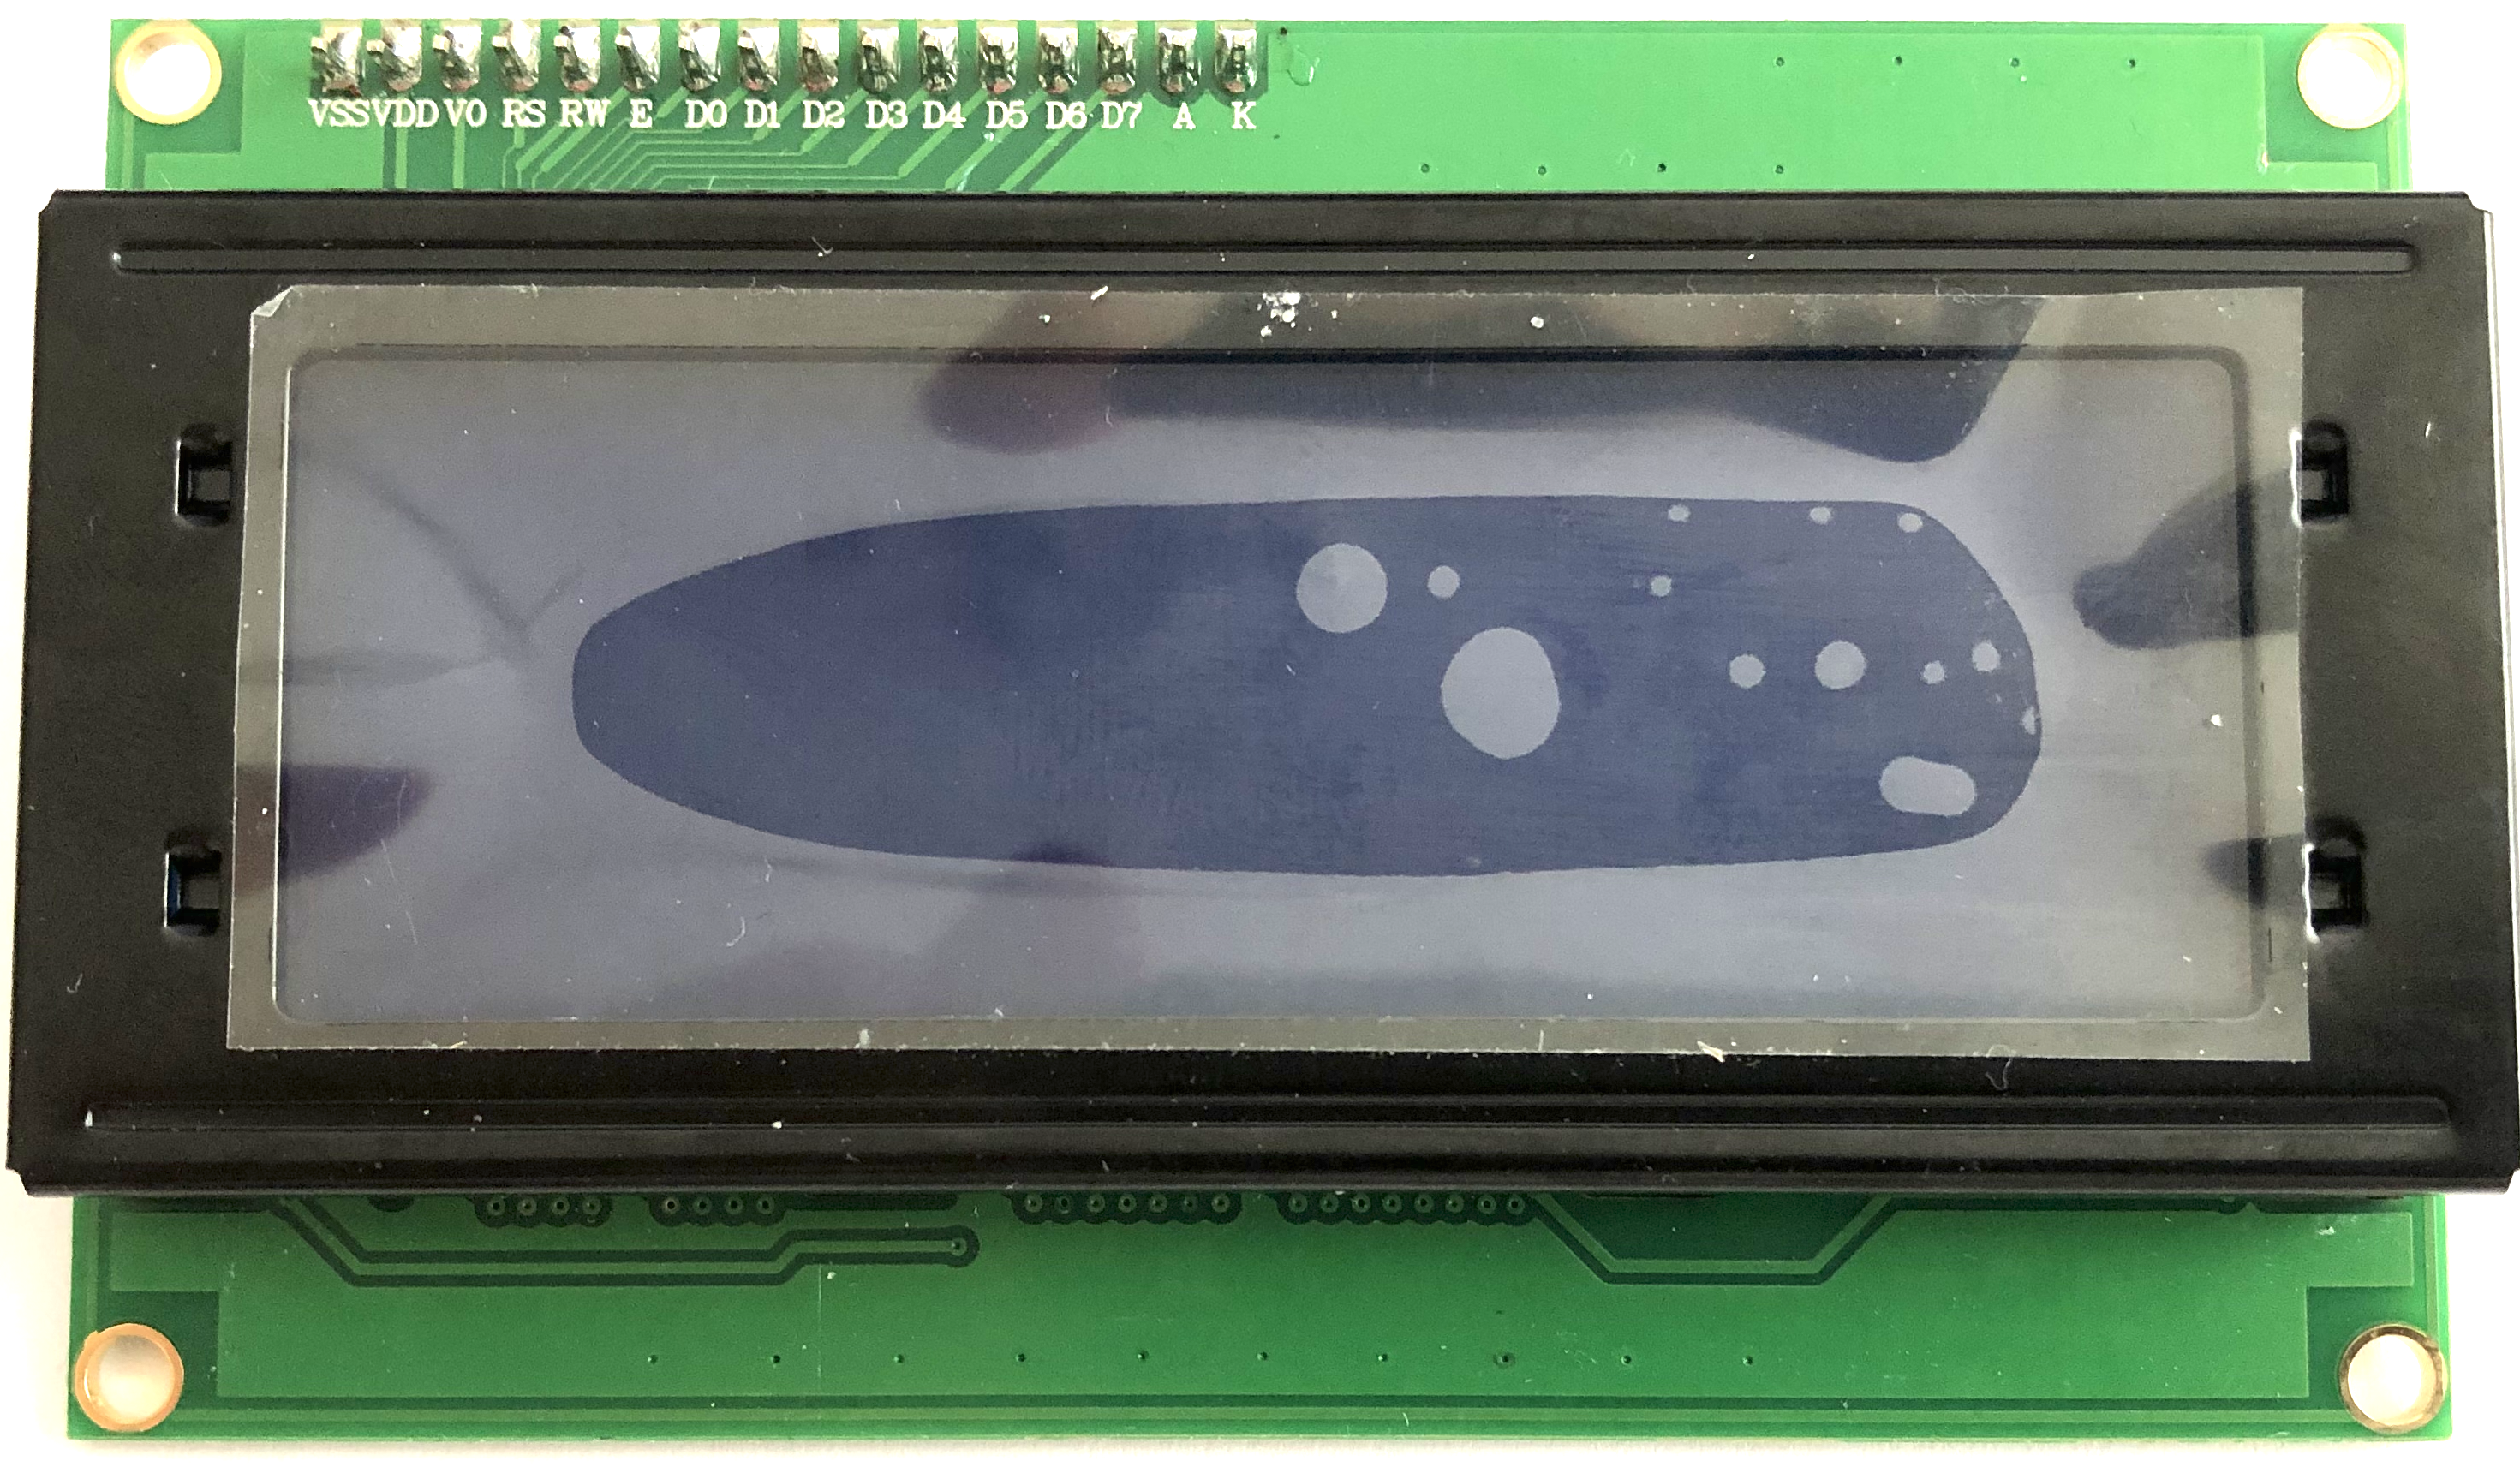
\includegraphics[height=.15\textheight]{LCD-Vorderseite}
		\caption{LCD-Modul Vorderseite}
		\label{fig:LCD-front}
	\end{minipage}
	\hfill
	\begin{minipage}{.45\linewidth}
		\centering
		\includegraphics[height=.15\textheight]{LCD-Rückseite}
		\caption{LCD-Modul Rückseite}
		\label{fig:LCD-back}
	\end{minipage}
\end{figure}
%Literatur: serielle und paralle Datenübertragung
Im Auslieferungszustand (Abbildung \ref{fig:LCD-front} und \ref{fig:LCD-back}) besteht das Modul aus einer großen grünen Platine mit dem fest verbauten LCD darauf und einem an die 16\,Pins gelöteten $I^2C$-Modul\footnote{Bussystem zur seriellen Übertragung von Daten \cite[S. 61]{MCU_in_Practice}} (kleine schwarze Platine), mit der das Beschreiben des Displays mittels serieller Übertragung möglich ist. Der Vorteil der seriellen Datenübertragung mittels $I^2C$ ist, dass nur eine Datenleitung, eine Taktleitung und das 0\,V-Potential mit dem MCU verbunden werden müssen. Einen Nachteil stellt die Übertragungsgeschwindigkeit dar, denn alle Bits müssen nacheinander übertragen werden. Geht man davon aus, dass die gleiche Taktrate bei einer parallelen Datenübertragung mit 8\,Bits erreicht wird, so ist die Übertragungsrate der seriellen Übertragung mindestens um den Faktor 8 kleiner, da zu den 8 zu übertragenen Bits eine Start-Bedingung des $I^2C$-Protokolls hinzukommt \cite[S. 62]{MCU_in_Practice}. Da die Geschwindigkeit der Übertragung von besonderer Bedeutung ist, wird das $I^2C$-Modul von dem Modul entfernt. Stattdessen wird die parallele 8-Bit Datenübertragung verwendet. Insgesamt werden elf Leiterbahnen vom LCD-Modul direkt zum MCU geführt. Die einzelnen Funktionen der Pins des LCD-Moduls können Tabelle \ref{tab:LCD_Pins} entnommen werden. Die Pin-Paare $VDD$/$VSS$ und $A$/$K$ werden jeweils mit dem 5\,V und 0\,V Potential der USB-Schnittstelle beschaltet. Pin $R/\overline{W}$ wird außerdem mit dem 0\,V Potential verbunden, da das LCD-Display ausschließlich vom MCU beschrieben und nicht gelesen werden soll. Die übrigen Pins werden direkt mit dem MCU verbunden. Der Kontrast des Display wird mit einer analogen Spannung an Pin $VO$ eingestellt, welche als pulsweitenmoduliertes Signal vom MCU ausgeht.
\begin{table}[h]
	\begin{center}
		\caption{LCD-Pinbelegung \cite[s. 7]{LCD_MN}}
		\begin{tabular}{l | l}
			\textbf{Pin} & \textbf{Funktion}\\
			\hline
			VDD \& VSS & generelle Spannungsversorgung\\
			A \& K & Anode und Kathode der LED-Hintergundbeleuchtung\\
			D0-D7 & Datenbus\\
			RS & H: Display Data, L: Display Instruction\\
			E & Enable\\
			R/W & Read/Write-Modus\\
			VO & LCD-Kontrast\\
		\end{tabular}
	\label{tab:LCD_Pins}
	\end{center}
\end{table}\\
Die Darstellung der Zeichen in den Punkt-Matrizen wird mithilfe von insgesamt drei Treiberchips realisiert. Die Treiberchips übersetzen die eingehenden Signale der acht Daten und  vier Steuerleitungen in entsprechende Funktionen, wie die Ausgabe eines bestimmten Zeichens oder das Leeren des gesamten Displayinhaltes. Eine Tabelle im Datenblatt des LCD-Moduls zeigt die Konstellationen von High- und Low-Pegeln der acht Datenleitungen und welche Zeichen daraus resultieren. Das Datenblatt befindet sich im Anhang \ref{CD-Anhang}.
%Auf den Aufbau inklusve Treiberchips eingehen? Ist die Frage ob das für die Funktion an sich überhaupt wichtig ist.
%\textbf{Aufbau des Moduls}\\
%Die Steuerung des Displays wird durch einem im Modul vebauten $SPLC780D$-Treiberchip und zwei $SPLC063$-Treiberchips realisiert.
%\hspace*{5mm}-HDxxx Chip\\
%\hspace*{10mm}-8-Bit / 4-Bit Modus\\
%\hspace*{10mm}-Adressplätze für (Position des Cursors?)\\
%\hspace*{10mm}-Schieberegister\\
%\hspace*{10mm}-Befehl geben\\
%\hspace*{10mm}-ASCII\\
%\hspace*{5mm}-Character Darstellung\\
% !TEX root = BA-Bauer.tex

\subsection{LED}

Licht emmittierende Dioden (LED) sind ein essentieller Bestandteil der Benutzerschnittstelle für die Lokaisierung von Fehlern und der Überwachung während einer Aufnahme- oder Wiedergabe aus kurzer und großer Distanz. Insgesamt werden fünf LEDs in vier verschiedenen Farben (blau, orange, grün und rot) verbaut um dem Benutzer eine Unterscheidung auch auf große Distanz zum Gerät möglichst einfach zu machen. Ziel ist eine möglichst hardwarenahe Rückmeldung an den Benutzer zu geben. Tabelle \ref{table:LED} fasst die Funktionen der einzelnen LEDs zusammen. 
\begin{table}[h]
	\begin{center}
		\caption{LED Funktionen}
		\begin{tabular}{l | l}
				\textbf{LED-Farbe} & \textbf{Funktion}\\
				\hline
				blau & Eingeschaltet bei aktiver Spannungsversorgung des Geräts\\
				rot & Zustandsänderung bei eingehendem DMX-Datenpaket\\
				blau & Zustandsänderung bei ausgehendem DMX-Datenpaket\\
				orange & Eingeschaltet bei Schreib- oder Lesevorgängen der SD-Karte\\
				grün & Allgemeine Zustandsanzeige
		\end{tabular}
		\label{table:LED}
	\end{center}
\end{table}
Die erste blaue LED wird direkt an die 5\,V Versorgungsspannung, ausgehend von der USB-Buchse, über einen Widerstand zur Strombegrenzung, angeschlossen. Dadurch kann sehr einfach festgestellt werden ob das Gerät mit Spannung versorgt wird, unabhängig von der Funktion der restlichen Schaltung. Die zweite blaue und die rote LED müssen zwangsläufig per Software geschaltet werden, da der XLR Ein- und Ausgang parallel verbunden sind. Eine Unterscheidung von ein- bzw. ausgehenden Datenpaket ist so nicht möglich. Zudem haben Tests gezeigt, dass das direkte Verbinden einer LED mit einer Datenleitung die LED nur kaum bis nicht sichtbar zum leuchten bringt. Gleiches gilt für die orange LED. In einer Weiterentwicklung des Gerätes kann z.B. mithilfe einer monostabilen Kippstufe, wie einem NE555 IC \cite{NE555}, welche den eingeschalteten Zustand einer LED verlängern kann, eine hardwarenähere Lösung realisiert werden.
\begin{figure}[h]
	\begin{center}
		\includegraphics[scale = 0.9]{led-Schaltung}
		\caption{LED Schaltung}
		\label{fig:LED-Schaltung}
	\end{center}
\end{figure}
Abbildung \ref{fig:LED-Schaltung} zeigt die Verschaltung der von dem MCU gesteuerten LEDs. Jede LED wird mit 5\,V Spannung versorgt. Jeweils ein Widerstand begrenzt den Strom um ein Durchbrennen der LED zu verhindern. Da für die vorhandenen LEDs keine Datenblätter verfügbar sind, werden alle Vorwiderstände mit 120\,Ohm dimensioniert. Das eigentliche Ein- und Ausschalten wird über jeweils einen Transistor realisiert. Die Basen des Transistoren werden mit jeweils einem Ausgang des MCUs verbunden. Der Benutzer soll die Möglichkeit besitzen die Helligkeit der LEDs je nach Anforderung zu verändern. Dazu werden die Kollektoren aller LED-Schalttransistoren auf den Emitter eines weiteren Transistors \textit{TB} geschaltet. Die Basis wird mit einem Ausgangaspin des MCUs verbunden, der mittels eines Timers ein Pulsweitenmoduliertes-Signal (PWM-Signal) ausgeben kann. Mihilfe einer Anpassung der Pulsweite kann so die Helligkeit aller LEDs reguliert werden. Je kürzer die Pulsweite ist, also je kürzer die LED eingeschlatet ist, so weniger hell erscheint sie. Die Frequenz des Pulsweitenoduliert Signals muss dabei so hoch sein, dass für das menliche Auge nicht mehr ersichtlich ist wann die LED leuchtet oder nicht.\\
%Hier noch mehr zu PWM schreiben. Verweis aus Kapitel Software/Einstellungen
%Dimensionierung der Vorwiderstände
%In der aktuellen Version des Aufnahmegerätes sind die Vorwiderstände aller LEDs pauschal mit 120\,Ohm dimensioniert, was in stark unterschiedlichen Helligkeiten der einzelnen LEDs resultiert. 
%\begin{figure}[h]
%	\begin{center}	
%		\includegraphics[width=\linewidth/4]{LED-Messung}
%		\caption{LED-Spannungsabfall Messung}
%	\end{center}
%\end{figure}
%
%\begin{table}[h]
%	\begin{center}
%		\begin{tabular}{l | l | l | l}
%			\textbf{LED-Farbe} & \textbf{$U_{LED}$} & $U_R$ & $I_{LED}$\\
%			\hline
%			blau & 3,9\,V & 0,7\,V & 5,83\,mA\\
%			rot & 2,0\,V & 2,6\,V & 21,66\,mA\\
%			grün & 2,5\,V & 1,9\,V & 15,83\,mA\\
%			orange & 2,2\,V & 2,4\,V & 20,00\,mA\\
%		\end{tabular}
%	\caption{Messung mit 120\,Ohm Vorwiderstand}
%	\end{center}
%\end{table}
% !TEX root = BA-Bauer.tex

\subsection{Spannungsversorgung}
Eine stabile und zuverlässige Spannungsversorgung ist für jede Schaltung besonders wichtig, denn die beste Schaltung funktioniert nicht ohne sie. Um eine großtmögliche Kompatibilität für den Benutzer zu gewährleisten, wird das Gerät über eine USB-Schnittstelle mit der nötigen Spannung versorgt. Dadurch kann das Gerät von mobilen Akkus oder USB-Netzteilen betrieben werden. Die nachstehende Tabelle zeigt den benötigten Versorgungsspannungs- und den Strombedarf der einzelnen Komponenten. 
\begin{table}[h]
	\begin{center}
		\caption{Spannungs- und Strombedarf}
		\begin{tabular}{l | c | r }
			\textbf{Bauteil} & \textbf{Versorgungsspannung} & \textbf{Strombedarf}\\
			\hline
			MCU & 1,7\,V - 3,6\,V & max. 240\,mA\\
			RS485 Treiberchip VDDA & 1,71\,V - 5,5\,V & max. 6,6\,mA\\
			RS485 Treiberchip VDDB & 4,5\,V - 5,5\,V (isoliert)& max. 12,5\,mA\\
			DC/DC Konverter & 4,5\,V - 5,5\,V & 28\,mA\\
			LCD-Modul & 3\,V - 10\,V & 100\,mA\\
			LED & 5\,V & ca. 20\,mA\\
			SD-Kartensteckplatz & 3,3\,V & -\\
			Encoder & 5\,V & -\\
			Taster & - & -\\
			\hline
			\textbf{Gesamt} & - & max. ca. 481\,mA
		\end{tabular}
	\label{tab:VDD+IDD}
	\end{center}
\end{table}
Die USB-Schnittstelle liefert laut der USB2.0-Spezifikation zwischen 4,75\,V und 5,5\,V \cite[S. 283]{USB-PD} und standardmäßig einen Strom von 100\,mA. Um mehr Strom von einem USB-Host\footnote{In der Hierarchie übergeordnetes USB-Gerät} anzufordern ist eine Kommunikation über die USB-Datenleitungen mithilfe eines Mikrocontrollers oder einem speziell für diesen Zweck vorgesehenen Chip notwendig. Allerdings kann das Gerät durch das Verbinden der beiden USB-Datenleitunen \textit{D+} und \textit{D-} mit einem Widerstand kleiner 200\,$\Omega$ als \textit{dedicated charging port} (DCP) vom USB-Host registriert werden \cite[S. 41]{USB-Battery}. Durch die Einstufung als DCP kann der USB-Host ohne jegliche Kommunikation bis zu 1,5\,A zur Verfügung stellen \cite[S. 45]{USB-Battery}. Als Stromversorgung können dann einfache USB-Netzteile, mobile -Batterien, -Anschlüsse an Laptops und PCs, sowie HUBs mit einer externen Stromversorgung genutzt werden.Voraussetzung für die Lieferung des Stroms ist eine ausreichend dimensionierte Stromversorgung des USB-Host selbst. 
\begin{figure}[h]
	\begin{center}
		\includegraphics[width=.8\linewidth]{Schaltung-power}	
		\caption{Schaltung Spannungsversorgung}
		\label{fig:Schaltung-power}
	\end{center}
\end{figure}
Abbildung \ref{fig:Schaltung-power} zeigt die Schaltung der Spannungsversorgung des Gerätes. Der Widerstand $R1$ sorgt dafür, dass das Gerät , wie bereits erwähnt, als DCP erkannt wird. Der Elektrolyt-Kondensator $C1$ fundiert als kleiner Puffer, falls die Schaltung für einen kurzen Moment mehr Strom benötigt als die USB-Schnittstelle liefern kann. Der damit einhergehende Spannungsabfall wird zudem kurzzeitig ausgeglichen. Um eventuell zurückfließenden Strom in den USB-Host zu verhindern wird die Diode $D1$ parallel zum 5\,V Potential (VCC) und Ground (GND) geschaltet. Auf der rechten Seite der Abbildung \ref{fig:Schaltung-power} befindet sich ein LDO-Spannungsregler. Er transformiert die eingehenden 5\,V vom USB-Host auf 3,3\,V herunter und stabilisiert diese gleichzeitig. Laut Tabelle \ref{tab:VDD+IDD} wird ein Strom von maximal ca. 240\,mA aus dem Spannungsregler benötigt. Laut Datenblatt fällt an ihm bei 25\,$^{\circ}$C Umgebungstemperatur und einem Strom von 250\,mA eine Spannung von ca. 100\,mV ab. Der MCU und der SD-Kartensteckplatz können somit mit ausreichend Spannung versorgt werden. Alle anderen Komponenten werden direkt mit den 5\,V der USB-Schnittstelle versorgt um den LDO-Spannungsregler so wenig wie möglich zu belasten.
% !TEX root = BA-Bauer.tex

\subsection{Autodesk EAGLE}
Die Schaltpläne und das Design der Platine wird in der \textit{Electronic Design Automation} (EDA) Software \textit{EAGLE} der Firma \textit{Autodesk} entwickelt. Innerhalb der Software können Schaltpläne erstellt werden. Anhand dieser Schaltung kann dann ein entsprechendes Layout der zu fertigenden Platine erstellt werden. Zuletzt können Produktionsdaten exportiert werden, mit denen die Platine industriell hergestellt werden kann \cite{eagle_homepage}.\\
Für die Erstellung des Schaltplans und Platinenlayouts wird eine Bauteilbibliothek benötigt. \textit{EAGLE} beinhaltet bereits initial eine große Bibliothek mit verschiedensten Bauteilen vieler Hersteller, jedoch umfasst die nicht alle am Markt verfügbaren Bauteile. Viele der in dieser Arbeit verwendeten Bauteile befinden sich nicht darin, weswegen eine eigene Bauteilbibliothek erstellt und explizit für die Entwicklung verwendet wird. Zudem soll dadurch das Fehlerrisiko in Bezug auf die Bauteilabmessungen und Pinbelegung reduziert werden. Ein Bauteil der Bauteilbibliothek besteht aus Sicht der Software aus drei Teilen. Dem $symbol$ (Abbildung \ref{fig:eagle-sym}), dem $footprint$ (Abbildung \ref{fig:eagle-foot}) und einem 3D-Modell (Abbildung \ref{fig:eagle-3d}).
\begin{figure}[h]
	\centering
	\begin{minipage}{.3\linewidth}
		\centering
		\includegraphics[height=.1\textheight]{lib-symbol}
		\caption{EAGLE Symbol}
		\label{fig:eagle-sym}
	\end{minipage}
	\hfill
	\begin{minipage}{.3\linewidth}
		\centering
		\includegraphics[height=.1\textheight]{lib-footprint}
		\caption{EAGLE Footprint}
		\label{fig:eagle-foot}
	\end{minipage}
	\hfill
	\begin{minipage}{.3\linewidth}
		\centering
		\includegraphics[height=.1\textheight]{lib-3d}
		\caption{EAGLE 3D-Modell}
		\label{fig:eagle-3d}
	\end{minipage}
\end{figure}
Das Symbol wird für die Entwicklung des Schaltplans verwendet und besitzt keine elektrischen Eigenschaften oder Dimensionen. Eine Simulation der Schaltung ist dementsprechend in $EAGLE$ nicht möglich. Die Anschlüsse der Symbole können im Schaltplan mit Leitungen verbunden werden. Um den Schaltplan auf die Hardwareebene zu projizieren, wird ein zugehöriger \textit{footprint} benötigt. Dieser enthält die Dimensionen und Anordnung der entsprechenden Lötstellen des Bauteils, welche in der Regel vom Hersteller des Bauteils zur Verfügung gestellt werden. Im Bibliotheks-Manager in \textit{EAGLE} werden dann die Anschlüsse des Symbols den entsprechenden Lötstellen des \textit{footprints} zugeordnet. Die Verbindung zwischen Schaltplan und Platine ist nun hergestellt. Um  einen noch realistischeren Entwurf der Platine einsehen zu können, kann ein 3D-Modell des Bauteils eingefügt werden. Standard Bauteile wie SMD-Kondensatoren, -Widerstände oder gängige Chip-Gehäuse können mit einem in \textit{EAGLE} integrierten Generator erzeugt werden. Mit den vom Hersteller des Bauteils angegebenen Dimensionen und Toleranzen erzeugt der Generator einen \textit{footprint} mit einem dazugehörigen 3D-Modell des Bauteils. Handelt es sich bei dem Bauteil nicht um ein Standard-Bauteil, so muss der \textit{footprint} in $EAGLE$ und das 3D-Modell in einer externen CAD-Software konstruiert werden. Über den Bibliotheks-Manager kann dann das 3D-Modell bezogen auf den \textit{footprint} dreidimensional platziert werden. Mithilfe der 3D-Modelle kann EAGLE in Verbindung mit der Software \textit{Fusion 360} der Firma \textit{Autodesk} ein 3D-Modell der gesamten Platine inklusive aller Bauteile, für die entsprechende 3D-Modelle in der Bauteilbibliothek existieren, exportieren. Dieses kann dazu verwendet werden, Kollisionen zwischen verschiedenen Bauteilen oder zwischen Bauteilen und Gehäuse vor der Fertigung der Platine zu erkennen oder ein passendes Gehäuse für die Platine zu entwerfen.\\
Mithilfe der in \textit{EAGLE} integrierten sogenannten \textit{Forward-Back-Annotation} werden Änderungen im Schaltplan unmittelbar in das Platinenlayout übertragen. Wird Beispielsweise nur der Wert eines Widerstandes im Schaltplan geändert, so ändert sich auch die Beschriftung des Bauteils auf der Platine. Außerdem werden in der Schaltung gesetzte Verbindungen im Platinenlayout dargestellt. Damit wird das Verlegen von Leiterbahnen vereinfacht und kann fehlerfrei durchgeführt werden. Im Schaltplan nicht bestehende Verbindungen können im Platinenlayout nicht hergestellt werden.
\begin{figure}[h]
	\centering	\begin{minipage}{.35\linewidth}
		\centering
		\includegraphics[height=.13\textheight]{Module}
		\caption{Modul $"$MAX$"$}
		\label{fig:module}
	\end{minipage}
	\hfill
	\begin{minipage}{.6\linewidth}
		\centering
		\includegraphics[height=.13\textheight]{Module-schematic}
		\caption{Inhalt des Moduls $"$MAX$"$}
		\label{fig:module-schematic}
	\end{minipage}
\end{figure}
Um die Schaltung möglichst übersichtlich zu gestalten, werden sogenannte \textit{Module} verwendet, durch die komplexe Schaltungen in kleinere \textit{$"$Black-Boxes$"$}\footnote{Box mit Ein-, Ausgängen und unbekanntem Inhalt} heruntergebrochen werden können. Abbildung \ref{fig:module-schematic} und \ref{fig:module} zeigen diese Vereinfachung. Zudem können Module mehrfach in einer Schaltung eingefügt werden. Änderungen in einem Modul wirken sich auf alle eingefügten aus. Verbindungen (grüne Linien in Abbildung \ref{fig:module-schematic}) zwischen Bauteilen werden Namen (\textit{net-names}) zugewiesen, die nur innerhalb des Moduls bekannt sind. Mithilfe der \textit{net-names} können sogenannte \textit{Ports} aus dem Modul herausgeführt werden, womit Verbindungen zu anderen Modulen oder einfachen Bauteilen hergestellt werden können. Pfeile an den $Ports$ signalisieren die Flussrichtung von Signalen, nicht vorhandene Pfeilspitzen signalisieren einen Anschluss einer Spannungsversorgung.\\
% !TEX root = BA-Bauer.tex

\subsection{Platinendesign} \label{sec:PCB-Design}
Das Design der Platine spielt eine wichtige Rolle in der Entwicklung des Gerätes, denn es müssen alle 78\,Komonenten auf ihr Platz finden, sie muss elektrisch und logisch sinnvoll aufgebaut sein und gleichzeitig kompakte Maße haben damit das Endprodukt handlich ist. Zudem kommen einige technische Anforderung von Bauteilen wie die Platzierung der Stützkondensatoren des MCUs, die möglichst nah an ihm platziert werden müssen, hinzu. Außerdem muss der SD-Karten-Steckplatz im nachhinein für den Benutzer zugänglich sein, der Benutzer muss die Taster betätigen, die LEDs leuchten, den LCD sehen können und in der Lage dazu sein die DMX- und das USB-Kabel in die entsprechenden Buchsen zu stecken.
\begin{figure}[h]
	\centering
	\begin{minipage}[t]{0.47\linewidth}
		\centering
		\includegraphics[width=\linewidth]{PCB_top}
		\caption{Platinenvorderseite}
		\label{fig:PCB-top}
	\end{minipage}
	\hfil
	\begin{minipage}[t]{0.47\linewidth}
		\centering
		\includegraphics[width=\linewidth]{PCB_bottom}
		\caption{Platinenrückseite}
		\label{fig:PCB-bottom}
	\end{minipage}
\end{figure}\\
Abbildung \ref{fig:PCB-top} und \ref{fig:PCB-bottom} zeigen das Layout der Platine als virtuelles dreidimensionales Modell. 
Auf der Platine werden zwei Arten von Komponenten verbaut. Zum Einen sogenannte \textit{surface-mount-technology}-Komponenten (SMT-Komponenten), zum Anderen \textit{through-hole technology}-Komponenten (THT- Komponenten). SMT-Komponenten werden direkt auf die Oberfläche der Platine gelötet, was keine Notwendigkeit von Löchern in der Platine erfordert. Durch die Oberflächenmotage befindet sich das Bauteil auf der selben Seite wie die dazugehörige Lötstelle. Für THT-Komponenten werden Löcher in der Platine benötigt, da die Pins der Komponenten im 90 Grad Winkel zur Oberfläche der Platine gerichtet sind. Diese können unter Umständen nur auf der gegenüberliegenden Seite der Platine verlötet werden. Eine LED zum Beispiel, die bündig mit der Platine verlötet werden soll, kann nur auf der gegenüberliegenden Seite der Platine verlötet werden, da die LED selbst ihre eigenen Pins verdeckt. Damit alle Komponenten frei auf der Platine platziert werden können, wird eine zweiseitige Platine entworfen. Diese besitzt auf der Vorder- und Rückseite eine Kupferschicht, welche mithilfe von sogenannten \textit{Vias}\footnote{Durchkontaktierte Löcher in der Platine} verbunden werden können.
\begin{figure}[h]
	\begin{center}
		\includegraphics[width=\linewidth]{PCB-Design_mark}
		\caption{Platinenlayout-Aufteilung}
		\label{fig:PCB-Layout}
	\end{center}
\end{figure}
Abbildung \ref{fig:PCB-Layout} zeigt die generelle Aufteilung der Platine. Diese Aufteilung vereinfacht die mögliche Fehlersuche und trägt dazu bei die Leiterbahnlängen zu verkürzen. Alle blau gefärbten $Pads$\footnote{In der Regel rechteckige Lötstellen (freigelegte Kupferflächen) zum verlöten von SMT-Komponenten} und Leiterbahnen befinden sich auf der Vorderseite, alle rot eingefärbten auf der Rückseite der Platine. Die freien Flächen zwischen den Leiterbahnen auf der Ober- und Unterseite sind mit dem 0\,V Potential verbunden. Die grünen Bohrungen sind $Vias$ und durchkontaktiert Bohrungen für die THT-Komponenten.
Der Formfaktor der Platine wird im wesentlichen von dem LCD-Modul vorgegeben, da es bei weitem das größte Bauteil darstellt. Neben dem LCD-Modul muss außerdem Platz für den Encoder, die Taster und LEDs vorhanden und für den Benutzer sichtbar und verwendbar sein. Aus diesem Grund werden das LCD-Modul, die Taster, der Encoder und die LEDs auf der Vorderseite der Platine platziert. Im Zentrum der Platine befindet sich das LCD-Modul. Unterhalb des Moduls befinden sich die Taster, rechts davon die LEDs. Die LED, die den Zustand der Spannngsversorgung anzeigt befindet sich oben links um eine Verwechslungen mit der zweiten blauen LED zu verhindern. Der SD-Kartensteckplatz, grün markiert, findet am linken Rand unterhalb der USB-Buchse und Schaltung der Spannungsversorgung, blau markiert, der Platine Platz. Der MCU bildet den größten Knotenpunkt der Schaltung und befindet sich deswegen in der Mitte der Platine. Laut Hersteller sollen die Stützkondensatoren möglichst nah am MCU plaziert werden, damit die Induktivität der Leiterbahnen den hohen Stromfluss aus den Kondensatoren heraus nicht beeinträchtigt, wie bereits in Kapitel \ref{sec:STM} erläutert. Kritische an den MCU angeschlossene Komponenten sind unter anderem der SD-Kartenslot, der Quartz und der RS485-Treiberchip. Um möglichst wenig Störungen auf die Leiterbahnen einwirken zu lassen sind diese möglichst kurz. Die XLR-Buchsen für die ein- und ausgehenden DMX-Daten befinden sich am oberen Rand der Rückseite der Platine. Sie und die Schaltung des Treiberchips, rot markiert, liegen nah beieinander um auch hier das Störungspotential durch lange Leiterbahnen möglichst gering zu halten.
% !TEX root = BA-Bauer.tex

\subsection{Gehäusedesign}
Mit dem Gehäuse wird aus der eher abstrakt wirkenden Platine ein optisch ansprechendes Endprodukt. Wichtig ist nicht nur die Optik, sondern auch das Design in funktioneller Sichtweise. Das beschriebene Platinendesign in Kapitel \ref{sec:PCB-Design} und das 3D-Modell bilden die Basis für die Entwicklung des Gehäuses. Diese können durch die Verbindung von $EAGLE$ mit der 3D-CAD-Software $Fusion360$  der Firma Autodesk direkt virtuell in die Konstruktion eingefügt werden. Damit kann sichergestellt werden, dass z.B. Bohrungen im Gehäuse mit den in der Platine befindlichen übereinstimmen und dass die Bauteile auf der Platine nicht mit dem Gehäuse kollidieren. Die Konstruktion ist auf die Fertigung im 3D-Druckverfahren ausgerichtet, da so in kurzer Zeit Design-Iterationen kostengünstig hergestellt werden können. Bei dem verwendeten Material handelt es sich um den biologisch abbaubaren Kunststoff $Poly-lactid-acid$ (PLA). Er ist einfach zu drucken, nachzubearbeiten, kostengünstig in der Anschaffung und besitzt eine ausreichende Stabilität.\\
Abbildung \ref{fig:Housing-front} und \ref{fig:Housing-back} zeigen das 3D-Modell des Gehäuses, dessen grundsätzliches Design simpel und kompakt ist (15,7\,cm breit, 8,14\,cm tief und 5,25\,cm hoch). Die Breite und Tiefe des Gehäuses werden nahezu komplett von der Platine ausgefüllt. Die Höhe des Gehäuses wird von den XLR-Buchsen vorgegeben und ist daher besonders im vorderen Teil nicht voll ausgenutzt. Bei einer Weiterentwicklung könnte dieser freie Platz für einen integrierten Akku genutzt werden. Der Boden des Gehäuses verläuft parallel zur Platine, damit die eingesteckten Kabel rechtwinklig zur Tischoberfläche verlaufen und sie somit das Gerät durch ihr Eigengewicht nicht zum Kippen bringen. Auf der Oberseite befindet sich ein rechteckiger Ausschnitt für das LCD-Modul, sowie runde Ausschnitte für die LEDs, Taster und den Encoder. Über den LEDs befinden sich weiße Diffusionsscheiben, die das Licht der darunterliegenden LEDs brechen. Somit ist das Leuchten aus größerer Distanz und anderen Blickwinkeln sichtbar. Auf der Rückseite befinden sich runde Ausschnitte für die XLR-Buchsen und eine Vielzahl von Schlitzen, die einen Luftaustausch ermöglichen und einem Hitzestau vorbeugen. Auf der linken Seite befinden sich Ausschnitte für den SD-Kartensteckplatz und den USB-Anschluss.
\begin{figure}[h]
	\begin{minipage}{.45\linewidth}
		\centering
		\includegraphics[height=.2\textheight]{Housing-front}
		\caption{Gehäuse 3D-Modell Frontseite}
		\label{fig:Housing-front}
	\end{minipage}
	\hfill
	\begin{minipage}{.45\linewidth}
		\centering
		\includegraphics[height=.2\textheight]{Housing-back}
		\caption{Gehäuse 3D-Modell Rückseite}
		\label{fig:Housing-back}
	\end{minipage}
\end{figure}
Die Platine muss ausreichend im Gehäuse befestigt sein, damit sie sich beim Betätigen der Taster nicht kurzzeitig verbiegt. Durch das kurzzeitige Verbiegen wird das Betätigen der Taster erschwert bzw. unmöglich gemacht und die Platine unter Umständen beschädigt. Abbildung \ref{fig:Housing-Befestigung} und \ref{fig:Housing-Befestigung2} zeigen Schnittanalysen des 3D-Modells. Für einen größtmöglichen Halt der Platine im Bereich der Taster wird die Platine in einen Schlitz im Gehäuse eingeführt (rot markiert). Durch den Schlitz wird die Auflagefläche der Platine im Gehäuse erhöht und die durch einen Tastendruck einwirkende Kraft auf sie verteilt. Auf der gegenüberliegenden Seite wird die Platine mit M3-Gewinde-Schrauben befestigt (blau markiert). Dazu befinden sich zylinderförmige Extrusionen an der Oberseite, die mittig eine Bohrung mit einem M3-Gewinde haben. Mit der grün markierten Bohrung wird das LCD-Modul mit den bereits vorhanden Löchern verschraubt. Abstandshalter zwischen LCD-Modul und Platine ermöglichen die Verschraubung von der Unterseite der Platine.
\begin{figure}[h]
	\begin{minipage}{.35\linewidth}
		\centering
		\includegraphics[height=.13\textheight, angle=180]{Housing-Schnitt-Befestigung-mark}
		\caption{Gehäuse Schnitt}
		\label{fig:Housing-Befestigung}
	\end{minipage}
	\hfill
	\begin{minipage}{.55\linewidth}
		\centering
		\includegraphics[height=.13\textheight, angle=180]{Housing-Schnitt-Befestigung2-mark}
		\caption{Gehäuse Schnitt Draufsicht}
		\label{fig:Housing-Befestigung2}
	\end{minipage}
\end{figure}
Damit die Platine im Gehäuse platziert und befestigt werden kann, muss das Gehäuse geöffnet werden können. Um bei der Entwicklung möglichst unkompliziert die Platine erreichen zu können, befindet sich ein Clip-Mechanismus an der Unterseite des Gerätes, mit dem der Boden einfach entfernt werden kann. Abbildung \ref{fig:Housing-clip-side} zeigt die Seitenansicht des Mechanismus. In der Oberseite des Gehäuses befinden sich rechteckige Aussparungen, in die die an der Unterseite befindlichen Clips einhaken können. Durch das verwendete 3D-Druckverfahren sind die Clips eine Schwachstelle der Konstruktion, da PLA verhältnismäßig spröde ist und die Clips beim Einhaken in die Aussparungen leicht gebogen werden müssen. Um das Material beim verbiegen weniger zu belasten, sind die Clips bis in den Boden hinein verlängert. Dadurch wird das Material auf eine längere Strecke hinweg gebogen und das Biegemoment somit verteilt.
\begin{figure}[h]
		\begin{minipage}{.45\linewidth}
		\centering
		\includegraphics[height=.15\textheight]{Housing-Schnitt-Clip}
		\caption{Gehäuse Clip-Mechanismus Schnittansicht frontal}
		\label{fig:Housing-clip}
	\end{minipage}
	\hfill
	\begin{minipage}{.45\linewidth}
		\centering
		\includegraphics[height=.15\textheight]{Housing-Schnitt-Clip-Seite}
		\caption{Gehäuse Clip-Mechanismus Schnittansicht}
		\label{fig:Housing-clip-side}
	\end{minipage}
\end{figure}\\
Einen wichtigen Bestandteil der Bedienbarkeit stellen die Taster dar. Abbildung \ref{fig:Housing-btn-front} und \ref{fig:Housing-btn} zeigen den Mechanismus zum Betätigen des Tasters als Schnittansicht des 3D-Modells. Die Körper mit der Kennzeichnung 1 sind das Gehäuse an sich, die Taster sind mit 4 gekennzeichnet. Unter den Tastern befindet sich die Platine. Im Gehäuse befinden sich vier nach unten gerichtete Führungen für einen beweglichen Zylinder, welcher mit 3 gekennzeichnet ist. Alle vier Zylinder sind miteinander verbunden, um die Stabilität zu erhöhen und ein Verkanten dieser mit der Führung zu verhindern. Für die Zylinder wird ein gummiartiges Material namens $TPU$ für den 3D-Druck verwendet, wodurch das Klicken des Tasters gedämpft wird. Die für den Benutzer sichtbaren beweglichen Taster-Flächen, gekennzeichnet mit 2, drücken den Zylinder bei einer Betätigung nach unten und diese wiederum betätigen den Taster. Auf den Tasterflächen befinden sich Extrusionen mit der Kennzeichnung der entsprechenden Funktion des jeweiligen Tasters. Dadurch kann der Taster optisch und haptisch wahrgenommen werden, was besonders an Orten mit schlechten Beleuchtungsverhältnissen wichtig ist.
%Formulierung: TPU wegen der Verbindung der Zylinder. Tasterdruck könnte mehrere Tasten betätigen
\begin{figure}[h]
	\begin{minipage}{.45\linewidth}
		\centering
		\includegraphics[width=\linewidth]{Housing-Schnitt-Button-front-crop-mark}
		\caption{Gehäuse Clip-Mechanismus}
		\label{fig:Housing-btn-front}
	\end{minipage}
	\hfill
	\begin{minipage}{.45\linewidth}
		\centering
		\includegraphics[width=\linewidth]{Housing-Schnitt-Button-crop}
		\caption{Gehäuse Clip-Mechanismus Schnittansicht}
		\label{fig:Housing-btn}
	\end{minipage}
\end{figure}\\
Alle konstruierten Komponenten, sowie das 3D-Modell der Platine befinden sich als $.stl$-Datei im Anhang \ref{CD-Anhang}.\\
\newline
\textbf{Optimierungsmöglichkeiten}\\
Das verwendete Material für das 3D-Druckverfahren ist, wie bereits erwähnt, verhältnismäßig spröde. Aus diesem Grund sind die Wände des Gehäuses dicker Konstruiert, als es für die Herstellung mit einem Spritzgussverfahren mit ABS-Kunststoff notwendig wäre. Durch die Dicke der Wände kann die SD-Karte durch den Schlitz im Gehäuse nur schwer erreicht werden. Durch eine Vergrößerung des Schlitzes oder eine Verringerung der Wanddicke kann dieses Problem gelöst werden. Außerdem ist der Mechanismus für die Taster optimierungsbedürftig. Die Verbindung der Tasterflächen ist zu steif, wodurch beim Betätigen eines Tasters der jeweilige benachbarte Taster betätigt werden kann. Durch die Konstruktion einzelner Tasterflächen für jeden Taster kann das Problem gelöst werden. 
%Formaterung überprüfen: Einige Bilder stehen nicht am richtigen Platz (durch Seitenumbruch)